\section{历史截图、旧标签与 padding 错误复盘}
\label{app:historical}

\subsection{两张终端截图为什么不能作为论文主表}

用户提供的第一张历史截图把 ``Ground Truth Real Methylation Ratio'' 显示为 16.59\%。这一数值可以被精确重构为
\begin{equation}
\frac{323}{1505+442}=16.5896\%,
\end{equation}
即 1505 个真实位点之外又计入 442 个 batch padding 位置。在阈值 0.6 时，截图的预测甲基率 13.15\% 对应 $256/1947$，所谓 total end-to-end accuracy 38.11\% 对应 $742/1947$。它们的分母都不是实际测试位点数。

\begin{figure}[H]
  \centering
  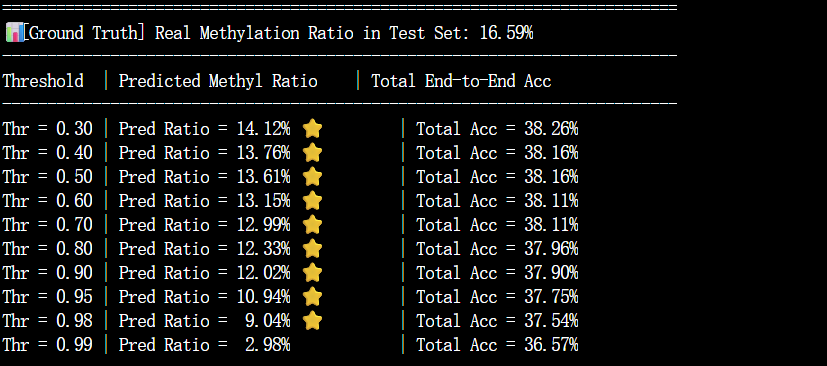
\includegraphics[width=0.94\textwidth]{supplementary/historical_padding_e2e_table.png}
  \caption{历史端到端阈值截图。该次运行的有效数组长度为 1947，其中 442 个为 padding，故比例不能用于论文。原始图片仅用于审计留档。}
  \label{fig:old-e2e}
\end{figure}

第二张截图可被另一种 batch 切分精确重构：有效数组长度为 $1505+386=1891$，正类仍是 323，padding 被当作阴性后阴性总数变成 1568。阈值 0.6 时混淆矩阵为 $TP=90$、$FP=38$、$TN=1530$、$FN=233$，从而得到截图中的 Accuracy 85.67\%、Precision 70.31\%、Recall 27.86\% 和 F1 39.91\%。若模型全部预测阴性，Accuracy 仍为
\begin{equation}
\frac{1568}{1891}=82.9191\%,
\end{equation}
正好对应截图在阈值 0.95--0.99 的 82.92\%。这说明结果会随 batch size 改变，而不是模型本身改变。

\begin{figure}[H]
  \centering
  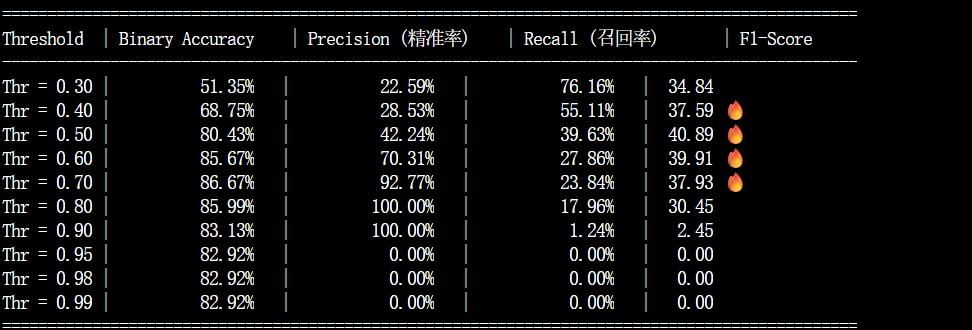
\includegraphics[width=0.94\textwidth]{supplementary/historical_padding_binary_table.png}
  \caption{历史二分类阈值截图。该次运行多计入 386 个 padding 阴性；所有显示值均可由错误混淆矩阵精确重构。}
  \label{fig:old-binary}
\end{figure}

根因是旧评价路径先按 padded batch 形状建立零初始化数组，再用不能排除这些有限零值的条件进入统计。padding 既没有真实残基，也没有合法甲基化标签，必须由真实长度/显式 mask 删除。附带的 \path{data/historical_padding_batch16_reconstruction.csv} 与 \path{data/historical_padding_batch8_reconstruction.csv} 保存了每个截图阈值的精确重构计数。

\subsection{去 padding 后，Ser 真值修正仍然必要}

只移除 padding、但继续使用旧 323 阳性标签时，已知序列 AUC 为 0.956，端到端 AUC 为 0.835；阈值 0.6 下，前者 Accuracy/Precision/Recall/F1 为 90.30\%/96.83\%/56.66\%/71.48\%，后者为 85.12\%/89.60\%/34.67\%/50.00\%。这些数值虽然已不受 padding 影响，但仍把 62 个本应为天然 Ser 的位点当作甲基阳性。

\begin{table}[H]
\centering
\caption{同一原始检查点在不同评价真值下的单体结果。阈值均为严格 $p>0.6$；旧标签只用于敏感性比较。}
\label{tab:label-sensitivity}
\begin{tabular}{L{30mm}L{31mm}rrrrr}
\toprule
真值版本 & 输入条件 & AUC & Accuracy & Precision & Recall & F1 \\
\midrule
旧 323 阳性 & 已知序列 & 0.956 & 90.30\% & 96.83\% & 56.66\% & 71.48\% \\
旧 323 阳性 & 端到端 & 0.835 & 85.12\% & 89.60\% & 34.67\% & 50.00\% \\
Ser 修正 261 阳性 & 已知序列 & 0.900 & 86.18\% & 64.02\% & 46.36\% & 53.78\% \\
Ser 修正 261 阳性 & 端到端 & 0.908 & 89.10\% & 88.80\% & 42.53\% & 57.51\% \\
\bottomrule
\end{tabular}
\end{table}

Ser 子集揭示了修正的影响：74 个 Ser 位点中只有 12 个为阳性；已知序列头在阈值 0.6 时把 74 个全部判为阳性，得到 $TP=12$、$FP=62$、$TN=0$、$FN=0$。因此，旧标签会把这 62 个系统性假阳性错误奖励为真阳性。正文采用修正后的 261/1244 真值，既不隐藏模型在 Ser 上的缺陷，也不因错误标签虚增性能。

\subsection{规划截图是指标清单，不是已完成数据}

\begin{figure}[H]
  \centering
  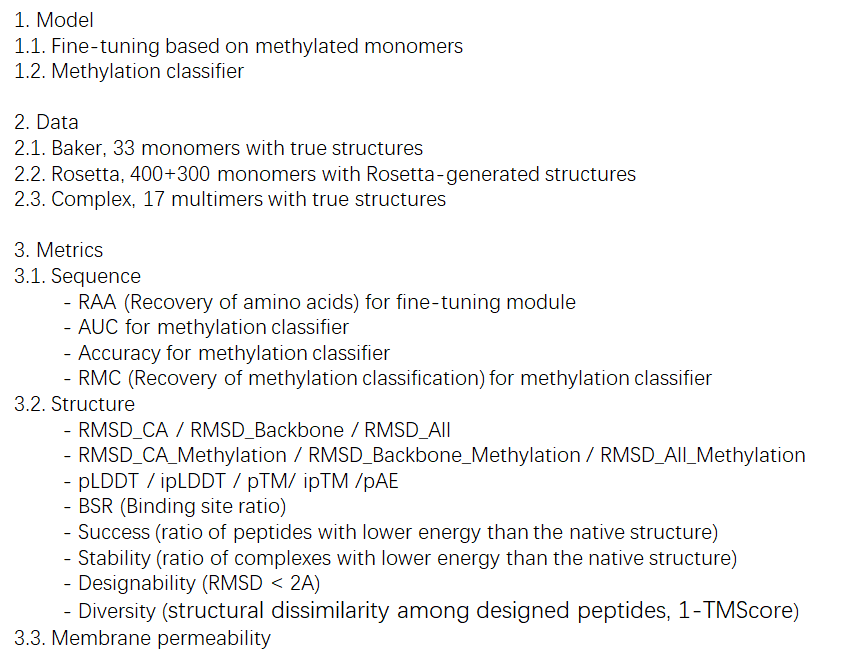
\includegraphics[width=0.92\textwidth]{supplementary/requested_metric_outline.png}
  \caption{尚哥提出的数据与指标规划截图。它定义了希望覆盖的项目，但不等于每项已经有原始结果；实际可用性逐项列于\cref{app:metric-matrix}。}
  \label{fig:metric-outline}
\end{figure}

截图中的 ``Baker, 33 monomers''、``Rosetta, 400+300 monomers'' 与冻结文件不一致。逐一审计 751 个原始 PDB 后，751/751 均含理论模型和 Rosetta 生成标记；406 个 \path{Me_} 对应 Rosetta-2023，345 个 \path{pdb_} 对应 Rosetta-2025。仓库、共享工作区与附件中均未找到可验证的 Baker 33 实验结构目录或清单。因此，本文采用“751 个 Rosetta 理论结构、600/151 划分”的可验证表述，不把规划截图冒充数据证据。

另有历史 V12 工作流的单体结构比较文件，但其检查点、结构队列和评价流程均不属于本文冻结的 V28 对象。为防止张冠李戴，本稿不移植其中任何数值；V28 单体结构指标仍明确标记为未计算。
